\chapter{Blood-Lines}
\label{cha:Lush_Chapter_25}
\index{Blood lines|(}

The word ``blood-line'' is often used by breeders and is found in
many advertisements and current animal breeding writings. It is rare,
however, in textbooks on animal breeding and still rarer in textbooks
on genetics.

In general, blood-line is synonymous with pedigree but is not so
definite. Sometimes it is used more nearly in one of the senses of family,
as, for example, when a man suggests performance testing of many
animals in a breed to find out ``which blood-lines are the most productive
and valuable,'' or wants to learn ``which are the most prominent
blood-lines of the breed.''

Sometimes blood-line is used to convey the idea of relationship, as
when a man says that two animals ``have nearly the same blood-lines,''
or that some animal ``has valuable blood-lines.'' In the first case he
implies that the two animals are closely related, and in the second case
he implies that this animal is closely related to some ancestors whose
descendants are highly valued. As a measure of relationship blood-line
is an indefinite and sometimes misleading substitute for the probability
of likeness which is expr,.essed accurately in the coefficient of relationship.
Usually it makes the relationship seem much higher than it really
is. Blood-line is a convenient term, however, because almost everyone
understands it in a general way.

Sometimes blood-line is used to describe a linebreeding or an
inbreeding program, as when a breeder says he ``believes in mating
together animals of similar but not identical blood-lines.'' He thus conveys
a vague idea of what would be more precise but probably not so
readily understood if he used the inbreeding coefficient and the relationship
coefficient to state how intensely he planned to inbreed and
how closely he was trying to keep his herd related to some noted
ancestor.

Sometimes blood-line is used to infer that a whole complex of inheritance
is transmitted as a unit unchanged from parent to offspring,
generation after generation. This idea comes from studying pedigrees
backward. The present famous animal is traced through his sire to a
grandsire and through it to a great grandsire, all of which were outstanding
individuals of their breed. Looking back to what happened,
we sometimes see an unbroken succession of outstanding merit. If we
could turn the pedigree around and look forward from the first famous
animal in the line, we might see what really happened. The outstanding
individual which was the first in this blood-line was used in one of
the leading herds of the breed. He had many sons and daughters; and,
as far as the breeder could pick them out, only the best of his sons were
saved for tentative use in leading herds, where they were mated to better-
than-average females. That son whose offspring proved him to be
the best became the leading sire of his generation and his supposedly
best sons were eagerly sought and in turn were tried out in the leading
herds of their time. This may have lasted several generations, or at least
as long as even one outstanding son of the outstanding sire in each generation
could be found. In a breed where one herd or a small group of
herds which get their sires from each other maintain a leading position
over many years, it sometimes happens that from grandsire to sire
and to son there was an unbroken succession of outstanding breed
leaders. This will become familiar to everyone who studies pedigrees of
that breed, and people will soon be referring to this as a ``very valuable
blood-line.'' Really what happened in such cases was nothing more fundamental
than an intense selection among the sons in each generation.
Because of its vagueness, blood-line is in bad repute as a scientific
word. Its claim to retention in the animal breeder's vocabulary is that it
is widely used now and that everyone understands -- at least in a general
way -- what is meant by it. The relationship coefficient and inbreeding
coefficient are not yet widely used and understood. They would
often require a long translation or explanation. There is no way to
make blood-line quantitative, but it is often useful where only a qualitative
meaning is necessary.

It is more nearly correct biologically to think of the individual as
one knot in an enormous network of descent, rather than as belonging
to some blood-line . The network is irregular in practically all respects
except that each individual has two and only two parents. Figure 44
shows a network which corresponds in a small way\footnote{Except that the
figure shows more inbreeding and hence more separation into
distinct families than is usual.} to the irregular and
interlocking lines of descent which constitute the pedigree structure of
a breed. Each small circle represents an individual, and the short
straight lines connect parent and offspring. Each individual's ancestry
widens out rapidly until, not many generations into the past, its
pedigree includes nearly the same animals as the pedigrees of its contemporaries
do, but with some ancestors repeated rarely and others repeated
many times. Some individuals leave many sons and daughters, others
few, and still others leave none. The breed is continuous in time and
space and changes but slowly. The individuals are discontinuous, and
each is different from all the others. Each individual is related to all the
others but in widely varying degiees. One blood-line can no qiore be
lifted out by itself than one strand of a fishing net could be picked up
without picking up all the others. Those nearest would be affected
soonest and most strongly. The fishing net, however, is much more regular
than the pedigree structure of a breed.

\begin{figure}
	\centering
    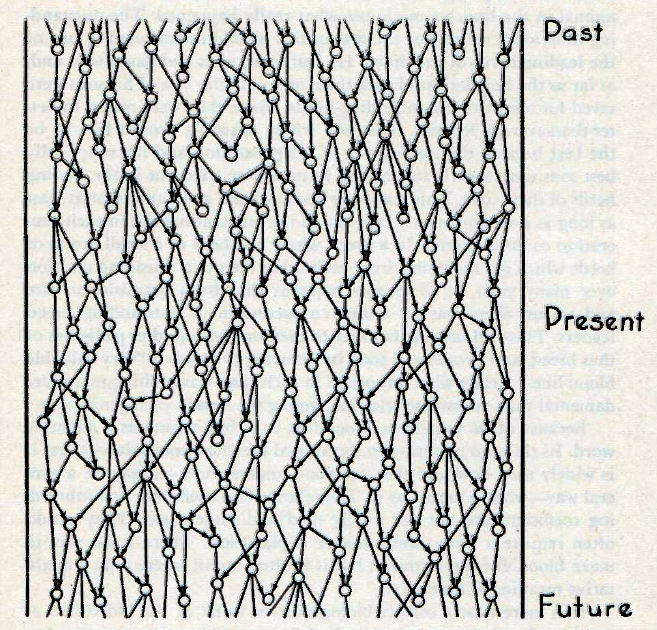
\includegraphics[width=\textwidth]{Figure_44.png}
    \caption{The pedigree of a population, showing that it is a network of descent
			 and is not composed of ``blood lines'' which are separate.}
    \label{fig:Lush_Figure_44}
\end{figure}

\section*{SUMMARY}

``Blood-line'' is an elastic term used sometimes as synonymous with
family, sometimes as a substitute for relationship, and sometimes to
describe vaguely a breeding system.

Because of its vagueness, blood-line is in bad repute as a scientific
term. But, because it is so widely understood by breeders, blood-line
will sometimes be found useful in conveying a general qualitative idea
about breeding topics where the speaker does not wish to call attention
to the quantitative aspect of that idea.
\index{Blood lines|)}

\newpage
\section*{REFERENCES}

\begin{hangparas}{0.5in}{1}%
\nowidow
Malin, D. F. 1923. The evolution of breeds. Des Moines: Wallace Publishing Company.
This book contains abundant references to blood and the word
``strain,'' or family. These show how one can speak more definitely on the
subject and yet avoid the use of ``blood-line.''

Whitney, Leon F. 1933. The basis of breeding. New Haven: E. C. Fowler. (Presents
many arguments against any use at all of ``blood'' to mean inheritance.)
\end{hangparas}